\chapter{Accuracy, Bandwidth and maximum current Verification} \label{App:AccuracyBWTest}
This appendix documents the test setups and test results for requirements §3, §4, §5 and §7 from the requirements in table \refq{tab:5_SystemRequirements} in chapter\refq{ch:SystemRequirements}.

\section{§3 Impedance Range Verification} \label{subsec:ZRangeVerify} 
The requirements states that instrument should be able to measure an impedance in the interval $10m\Omega < |Z| < 100M \Omega$. To test this requirement, the instrument is tested in both extremes of this range. An impedance reference, or precision calibrator, is not available for the project to use so a \SIQ{100}{\mega\ohm} resistor and a \SIQ{10}{\milli\ohm} resistor was made by placing multiple resistors in series/parallel.

\subsection{Verify \SIQ{100}{\mega\ohm} resistor and \SIQ{10}{\milli\ohm} resistor}

The \SIQ{100}{\mega\ohm} resistor is a series connection of 10 \SIQ{10}{\mega\ohm} resistors. The actual resistance must be known before testing the instrument. No available multimeter, or other instrument, was available to measure this, instead several DC power supplies are placed in series to supply \SIQ{320}{\volt}DC and the current through the resistor is measured with a 34401A DMM while the voltage across it is measured with another 34401 as seen on figure \refq{fig:App_A_Z_100MEGSetup}.

\begin{figure}[H]
    \centering
    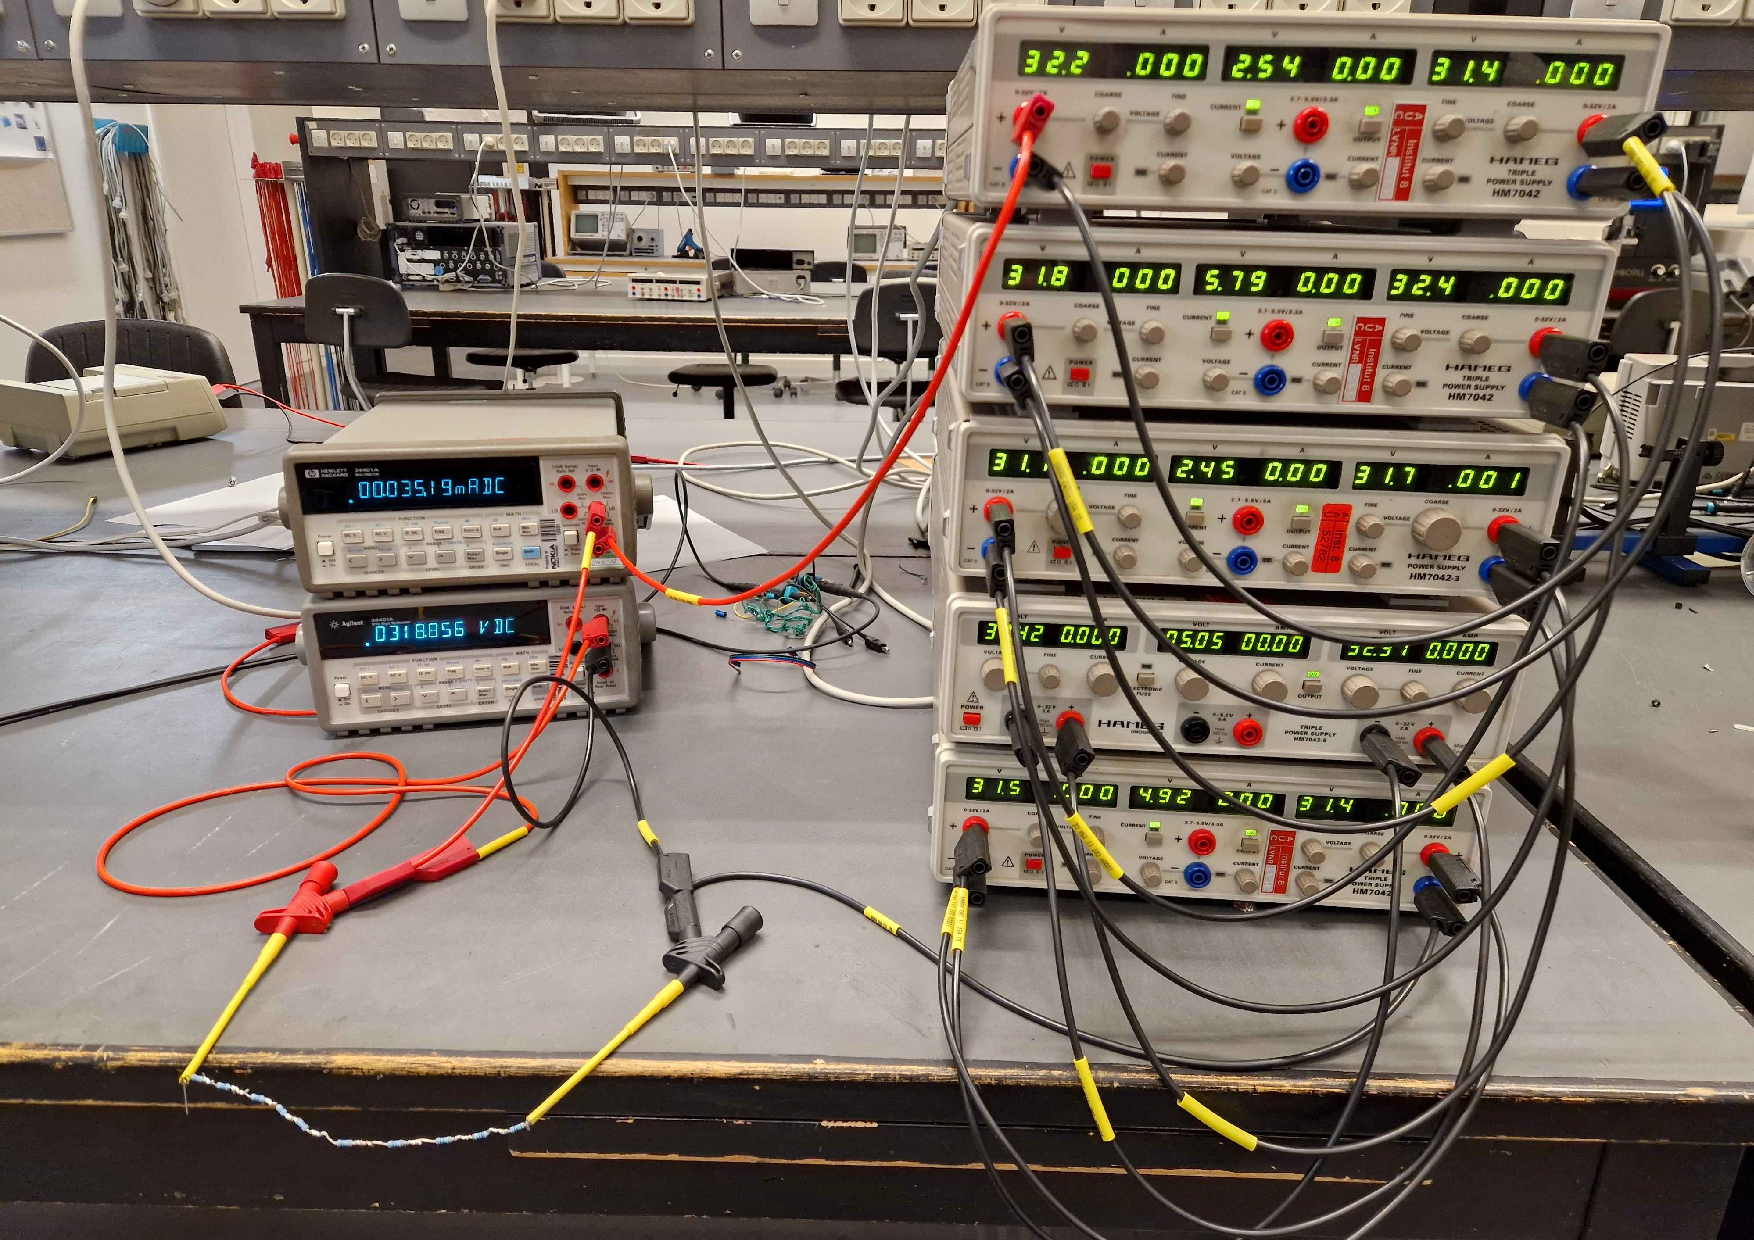
\includegraphics[clip, trim=0 0 0 0, width=0.75\textwidth]{Appendix/Figures/A_Z_100MegSetup.pdf}
    \caption{Several DC power supplies is set in series to produce 320VDC. The current through the resistor and the voltage across it is measured with two DMMs.}
    \label{fig:App_A_Z_100MEGSetup}
\end{figure}

The voltage across the resistor is $V_R = \SIQ{318.86}{\volt}$ while the current through it is $I_R = \SIQ{35.19}{\micro\ampere}$. The input impedance of the current measuring DMM is neglible while the voltage measuring DMM has an input impedance of \SIQ{10}{\mega\ohm}. The resistance is $R_{100M} = \SIQ{96.5}{\mega\ohm}$ as shown in eq \refq{eq:A_Z_100MegTest}.

\begin{equation}\label{eq:A_Z_100MegTest}
    \begin{split}
        \frac{V_R}{I_R} = ((Z_{INDMM})^{-1} + (R_{100M})^{-1})^{-1}\\
        R_{100M} = \frac{V_R Z_{INDMM}}{I_R Z_{INDMM}-V_R}\\
        R_{100M} = \frac{318.86 \cdot 10E6}{(35.18E-6)(10E6) + 318.86} = 9.6507E7
    \end{split}
\end{equation}

THe \SIQ{10}{\milli\ohm} resistor is a parallel connection of 10 \SIQ{100}{\milli\ohm} resistors. This resistor was also verified by letting a DC current pass through it and measuring the voltage across it. The test setup can be seen on figure \refq{fig:App_A_Z_100MilliSetup}.

\begin{figure}[H]
    \centering
    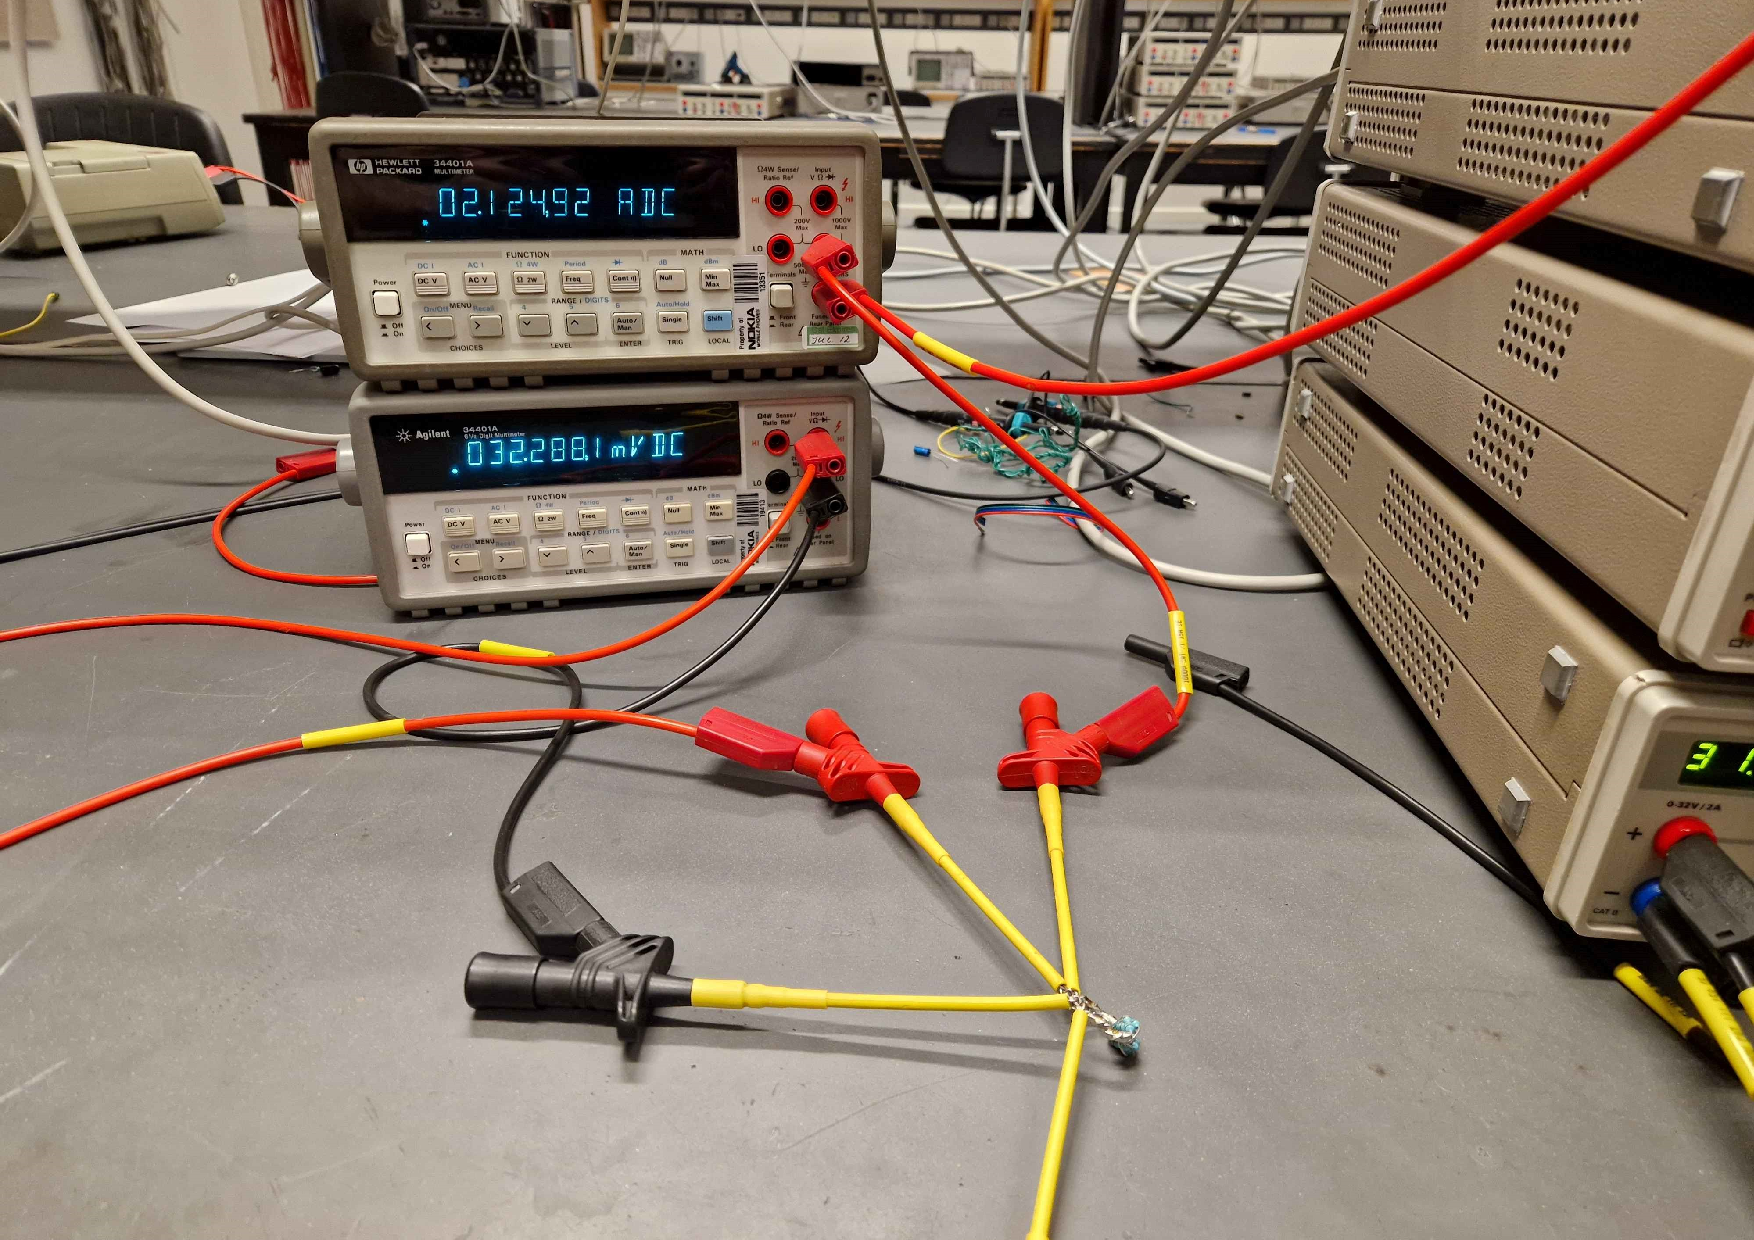
\includegraphics[clip, trim=0 0 0 0, width=0.75\textwidth]{Appendix/Figures/A_Z_10MilliSetup.pdf}
    \caption{A DC power supply is connected to the \SIQ{10}{\milli\ohm} resistor and the current through and voltage across it is measured with two DMMS.}
    \label{fig:App_A_Z_100MilliSetup}
\end{figure}

The voltage across the resistor is $V_{10MIL} = \SIQ{32.2881}{\milli\volt}$ the current through it is $I_{10MIL} = \SIQ{2.12492}{\ampere}$ so the resistor has a value of $R_{10MIL} =\SIQ{15.195}{\milli\ohm}$.

\subsection{Test results}

The $R_{100MEG} = \SIQ{96.5}{\mega\ohm}$ and $R_{10MIL} =\SIQ{15.195}{\milli\ohm}$ resistors have been measured by the instrument and the results can be seen in table \refq{tab:A_Z_ZRANGE_RESULT_TAB}. 

\begin{table}[H]
    \centering
    \renewcommand{\arraystretch}{1.5}
    \setlength{\tabcolsep}{8pt}
    \begin{tabular}{|c|c|c|c|c|c|}
    \hline
    \textbf{Resistor} & \textbf{Nom. Value} & \textbf{Meas. Value} & \textbf{Deviation} & \textbf{Requirement} & \textbf{Verdict} \\ \hline
    $R_{10MIL}$ & \SIQ{15.195}{\milli\ohm} & \SIQ{14.978}{\milli\ohm} & 1.428\% & $\pm$ 2\% & Pass  \\ \hline
    $R_{100MEG}$ & \SIQ{96.5}{\mega\ohm} & \SIQ{98.63}{\mega\ohm} & -2.207\% & $\pm$2\% & Fail \\ \hline
    \end{tabular}
    \caption{Test results for the measurements. The Nom. Value is the confirmed values of the test resistors. The Measured Value is the reading from the impedance analyzer. }
    \label{tab:A_Z_ZRANGE_RESULT_TAB}
    \end{table}

    The \SIQ{10}{\milli\ohm} range is passed, while the \SIQ{100}{\mega\ohm} range is failed as per for the requirement.  

    \section{§4, §5 Modulus and Phase Accuracy Verification on Mixed Impedance Types} \label{subsec:ModulusAccuracyTest} 

    The accuracy of the impedance has been measured at various test frequencies. The DUTs for this test will be \SIQ{10}{\ohm}, \SIQ{10}{\kilo\ohm} and \SIQ{100}{\kilo\ohm}. Capacitors were also tested, their values are \SIQ{27}{\pico\farad},\SIQ{150}{\nano\farad} and \SIQ{1}{\micro\farad}. An inductor was also tested it has the value \SIQ{100}{\micro\henry}.
    
    In the test result tables the abbreviations are the following. Tol. is tolerance of the component. Dev. M is deviation of module. Dev. Arg is deviation of argument. 

    The results for the resistors can be seen in table \refq{tab:A_Z_ImpedanceMeasurementWIthResistor}. The resistors are assumed to be ideal, so the phase is assumed to be $0\degree$ any deviation from this is an error.

        \begin{table}[H]
            \centering
            \renewcommand{\arraystretch}{1.5}
            \setlength{\tabcolsep}{8pt}
            \begin{tabular}{|c|c|c|c|c|c|c|}
            \hline
            \textbf{Resistor} & \textbf{Tol.} & \textbf{Meas. Z Value} & \textbf{Act. Res.} & \textbf{Dev. M} & \textbf{Dev. Arg} & \textbf{Freq} \\ \hline
            \SIQ{10}{\ohm} & 0.1\% & $9.9972 \angle -0.0091\degree$ & 9.9972 & 0.0256\% & $-0.0091\degree$ & \SIQ{1}{\kilo\hertz} \\ \hline
            \SIQ{10}{\ohm} & 0.1\% & $1.0000E1 \angle -0.4845\degree$ & 1.0000E1 & 0\% & $-0.4845\degree$ & \SIQ{50}{\kilo\hertz} \\ \hline
            \SIQ{10}{\ohm} & 0.1\% & $9.9968 \angle -1.4369\degree$ & 9.9968 & 0.032\% & $-1.4369\degree$ & \SIQ{250}{\kilo\hertz} \\ \hline
            \SIQ{10}{\kilo\ohm} & 0.1\% & $9.9974E3 \angle 0.0008\degree$ & 9.9974E3 & 0.026\% & $0.0008\degree$ & \SIQ{1}{\kilo\hertz} \\ \hline
            \SIQ{10}{\kilo\ohm} & 0.1\% & $9.9998E3 \angle -0.2289\degree$ & 9.9998E3 & 0.002\% & $-0.2289\degree$ & \SIQ{50}{\kilo\hertz} \\ \hline
            \SIQ{10}{\kilo\ohm} & 0.1\% & $9.9996E3 \angle -3.1832\degree$ & 9.9996E3 & 0.004\% & $-3.1832\degree$ & \SIQ{250}{\kilo\hertz} \\ \hline
            \SIQ{100}{\kilo\ohm} & 0.1\% & $1.0002E5 \angle -0.0045\degree$ & 1.0002E5 & -0.02\% & $-0.0045\degree$ & \SIQ{1}{\kilo\hertz} \\ \hline
            \SIQ{100}{\kilo\ohm} & 0.1\% & $9.9860E4 \angle -0.6684\degree$ & 9.9860E4 & 0.14\% & $-0.6684\degree$ & \SIQ{50}{\kilo\hertz} \\ \hline
            \SIQ{100}{\kilo\ohm} & 0.1\% & $1.0159E5 \angle -3.0477\degree$ & 1.0159E5 & -1.59\% & $-3.0477\degree$ & \SIQ{250}{\kilo\hertz} \\ \hline
            \end{tabular}
            \caption{Resistor Measurements at various test frequencies. The tolerance is the tolerance that the manufacturer has listed for the component.}
            \label{tab:A_Z_ImpedanceMeasurementWIthResistor}
        \end{table}
        

        The results for the Capacitors can be seen in table \refq{tab:A_Z_ImpedanceMeasurementWIthCapacitor}. It is assumed that the ESR of the capacitors is zero. The impedance that is used for calculating the deviation will simply be the capacitive reactance of each capacitor, $X_C = 1/(\omega C)$. The ideal angle of the impedance is assumed to be $-90\degree$. 
        
            \begin{table}[H]
                \centering
                \renewcommand{\arraystretch}{1.5}
                \setlength{\tabcolsep}{8pt}
                \begin{tabular}{|c|c|c|c|c|c|c|}
                \hline
                \textbf{Capacitor} & \textbf{Tol.} & \textbf{Meas. Z Value} & \textbf{Dev. M} & \textbf{Dev. Arg} & \textbf{Freq.} \\ \hline
                \SIQ{27}{\pico\farad} & 2\% & $5.8441E6 \angle -89.9512\degree$ & -0.865\% & $-0.0488\degree$ & \SIQ{1}{\kilo\hertz} \\ \hline
                \SIQ{27}{\pico\farad} & 2\% & $1.1779E5 \angle -90.0712\degree$ & 0.0890\% & $0.0712\degree$ & \SIQ{50}{\kilo\hertz} \\ \hline
                \SIQ{27}{\pico\farad} & 2\% & $2.3445E4 \angle -90.6537\degree$ & 0.5026\% & $0.6537\degree$ & \SIQ{250}{\kilo\hertz} \\ \hline
                \SIQ{150}{\nano\farad} & 1\% & $1.0662E3 \angle -90.0170\degree$ & -0.4870\% & $0.017\degree$ & \SIQ{1}{\kilo\hertz} \\ \hline
                \SIQ{150}{\nano\farad} & 1\% & $2.1294E1 \angle -90.2847\degree$ & -0.3456\% & $0.2847\degree$ & \SIQ{50}{\kilo\hertz} \\ \hline
                \SIQ{150}{\nano\farad} & 1\% & $4.2424 \angle -91.3710\degree$ & -0.041\% & $1.3710\degree$ & \SIQ{250}{\kilo\hertz} \\ \hline
                \SIQ{1}{\micro\farad} & 1\% & $1.5873E2 \angle -89.9869\degree$ & 0.2670\% & $-0.0131\degree$ & \SIQ{1}{\kilo\hertz} \\ \hline
                \SIQ{1}{\micro\farad} & 1\% & $3.1729 \angle -90.3050\degree$ & 0.3204\% & $0.3050\degree$ & \SIQ{50}{\kilo\hertz} \\ \hline
                \SIQ{1}{\micro\farad} & 1\% & $6.4554E-1 \angle -91.8117\degree$ & -1.382\% & $1.8117\degree$ & \SIQ{250}{\kilo\hertz} \\ \hline
                \end{tabular}
                \caption{Capacitor Measurements at various test frequencies. The tolerance is the tolerance that the manufacturer has listed for the component.}
                \label{tab:A_Z_ImpedanceMeasurementWIthCapacitor}
            \end{table}


            The results for the inductor can be seen in table \refq{tab:A_Z_ImpedanceMeasurementWIthInductor}. It is assumed that the ESR of the inductor is zero. The impedance that is used for calculating the deviation will simply be the inductive reactance of the inductor $X_L = \omega L$. The ideal angle of the impedance is assumed to be $90\degree$. 

                \begin{table}[H]
                    \centering
                    \renewcommand{\arraystretch}{1.5}
                    \setlength{\tabcolsep}{8pt}
                    \begin{tabular}{|c|c|c|c|c|c|}
                    \hline
                    \textbf{Inductor} & \textbf{Tol.} & \textbf{Meas. Value} & \textbf{Dev. M} & \textbf{Dev. Arg} & \textbf{Freq.} \\ \hline
                    \SIQ{100}{\micro\henry} & 5\% & $8.962E-1 \angle 43.3721\degree$ & $-42.6347\%$ & $46.6279\degree$ & \SIQ{1}{\kilo\hertz} \\ \hline
                    \SIQ{100}{\micro\henry} & 5\% & $3.0463E1 \angle 88.3468\degree$ & $3.0333 \%$ & $1.6532\degree$ & \SIQ{50}{\kilo\hertz} \\ \hline
                    \SIQ{100}{\micro\henry} & 5\% & $1.5216E2 \angle 87.796\degree$ & $-3.913 \%$ & $2.2040\degree$ & \SIQ{250}{\kilo\hertz} \\ \hline
                    \end{tabular}
                    \caption{Inductor Measurements at various test frequencies. The tolerance is the tolerance that the manufacturer has listed for the component.}
                    \label{tab:A_Z_ImpedanceMeasurementWIthInductor}
                \end{table}

                The inductor measurement at $f_{test} = 1kHz$ will be disregarded as the ESR of the inductor is substantial and cannot be ignored at this frequency.

\section{§4, §5 Modulus and Phase Accuracy Verification on Resistive Impedance Types} \label{subsec:ModulusAccuracyTest_res} 
Section \refq{subsec:ModulusAccuracyTest} tests the instrument at idearly purely capacitive, resistive and inductive elements. One limitation here is however that both capacitors and inductors are not know to better than \SIQ{1}{\%} at most. Furthermore the assumption of perfect Q does not hold in reality. While the used capacitors are high quality PP capacitors from the Vishay MKP1839 series, they will at some frequencies have a large loss, especially the \SIQ{1}{\micro\farad}.

The used resistors are \SIQ{0.1}{\%} thin film resistors from Vishay with a temperature coeffecient of less than \SIQ{15}{ppm}. These are assumed to be much more stable with frequency than both the capacitors and inductors. It is also assumed that they are AC-DC stable. This is very much not the case in reality, but no metrology grade references where available at the time.

The \SIQ{1}{\ohm} resistor is a \SIQ{0.5}{\%} \SIQ{100}{ppm} temperature coeffecient film resistor from Vishay/Dale. All used resistors are film type resistors, as they offer excelent AC performance. A \SIQ{15}{\milli\ohm} (idearly \SIQ{10}{\milli\ohm}) resistor is also used. This resistor has been verified using two HP/Keysight 34401 DMMs at DC. It is assumed to have a good AC-DC stability, see above section for verification.

Based on these assumptions a purely resistive test has been conducted. One that measures a wide range of resistors at \SIQ{1}{\kilo\hertz}, and one that measures a \SIQ{1}{\kilo\ohm} resistor at different frequencies. The maximum test frequency is \SIQ{300}{\kilo\hertz} as the system is not yet developed to utilize the full \SIQ{1}{\mega\hertz} analog front end Bandwidth.


\begin{table}[H]
    \centering
    \renewcommand{\arraystretch}{1.5}
    \setlength{\tabcolsep}{8pt}
    \begin{tabular}{|c|c|c|c|c|c|c|}
    \hline
    \textbf{Resistor} & \textbf{Tol.} & \textbf{Meas. Z Value} & \textbf{Dev. M} & \textbf{Dev. Arg} & \textbf{Freq} \\ \hline
    \SIQ{0.0152}{\ohm} & 0.134\% & $0.0148 \angle 0.1501\degree$  & -2.632\% & $0.0148\degree$ & \SIQ{1}{\kilo\hertz} \\ \hline
    \SIQ{1}{\ohm} & 0.5\% & $1.0015 \angle -0.0296\degree$  & 0.150\% & $-0.0296\degree$ & \SIQ{1}{\kilo\hertz} \\ \hline
    \SIQ{10}{\ohm} & 0.1\% & $9.9957 \angle -0.0085\degree$ & -0.043\% & $-0.0086\degree$ & \SIQ{1}{\kilo\hertz} \\ \hline
    \SIQ{100}{\ohm} & 0.1\% & $100.04 \angle -0.0073\degree$ &  0.040\% & $-0.0073\degree$ & \SIQ{1}{\kilo\hertz} \\ \hline
    \SIQ{1}{\kilo\ohm} & 0.1\% & $1.0001E3 \angle -0.0054\degree$ &  0.010\% & $-0.0054\degree$ & \SIQ{1}{\kilo\hertz} \\ \hline
    \SIQ{10}{\kilo\ohm} & 0.1\% & $10.002E3 \angle -0.0044\degree$ &  0.020\% & $-0.0044\degree$ & \SIQ{1}{\kilo\hertz} \\ \hline
    \SIQ{100}{\kilo\ohm} & 0.1\% & $99.959E3 \angle -0.0093\degree$ & -0.041\% & $-0.0093\degree$ & \SIQ{1}{\kilo\hertz} \\ \hline
    \SIQ{1}{\mega\ohm} & 0.1\% & $1.0009E6 \angle -0.0160\degree$ & 0.090\% & $-0.0160\degree$ & \SIQ{1}{\kilo\hertz} \\ \hline
    \end{tabular}
    \caption{Various resistor measurements at \SIQ{1}{\kilo\hertz}. The tolerance is the tolerance that the manufacturer has listed for the component, except for the \SIQ{15}{\milli\ohm}, this is verified in section \refq{subsec:ZRangeVerify}.}
    \label{tab:A_Z_ImpedanceMeasurementWIthResistor_Res_1KHZ}
\end{table}

\begin{table}[H]
    \centering
    \renewcommand{\arraystretch}{1.5}
    \setlength{\tabcolsep}{8pt}
    \begin{tabular}{|c|c|c|c|c|c|c|}
    \hline
    \textbf{Resistor} & \textbf{Tol.} & \textbf{Meas. Z Value} & \textbf{Dev. M} & \textbf{Dev. Arg} & \textbf{Freq} \\ \hline
    \SIQ{1}{\kilo\ohm} & 0.1\% & $1.0000E3 \angle -0.0012\degree$ &  0.000\% & $-0.0012\degree$ & \SIQ{0.1}{\kilo\hertz} \\ \hline
    \SIQ{1}{\kilo\ohm} & 0.1\% & $1.0001E3 \angle -0.0054\degree$ &  0.010\% & $-0.0054\degree$ & \SIQ{1}{\kilo\hertz} \\ \hline
    \SIQ{1}{\kilo\ohm} & 0.1\% & $1.0002E3 \angle -0.0692\degree$ &  0.020\% & $-0.0692\degree$ & \SIQ{10}{\kilo\hertz} \\ \hline
    \SIQ{1}{\kilo\ohm} & 0.1\% & $0.9992E3 \angle -0.4027\degree$ &  -0.080\% & $-0.4027\degree$ & \SIQ{100}{\kilo\hertz} \\ \hline
    \SIQ{1}{\kilo\ohm} & 0.1\% & $1.0006E3 \angle -1.2391\degree$ &  0.060\% & $-1.2391\degree$ & \SIQ{300}{\kilo\hertz} \\ \hline
    \end{tabular}
    \caption{\SIQ{1}{\kilo\ohm} at various frequencies. The tolerance is the tolerance that the manufacturer has listed for the component.}
    \label{tab:A_Z_ImpedanceMeasurementWIthResistor_FRQ_1KOHM}
\end{table}


\section{§7 Maximum Test Current} \label{subsec:MaxCurrent}
This section describes how the developed system is tested, to see if it can deliver more than the required \SIQ{100}{\milli\ampere}$_{pp}$ required.

A \SIQ{1}{\ohm} resistor is connected as in figure \ref{fig:App_MaxCurrent}. The used resistor has a tolerance of \SIQ{0.5}{\%}. The Impedance Analyzer is configured for \SIQ{2.3}{\volt}$_{pp}$ \SIQ{1}{\kilo\hertz} test signal. The voltage across the resistor is then measured using a HP34401A multimeter.

\begin{figure}[H]
    \centering
    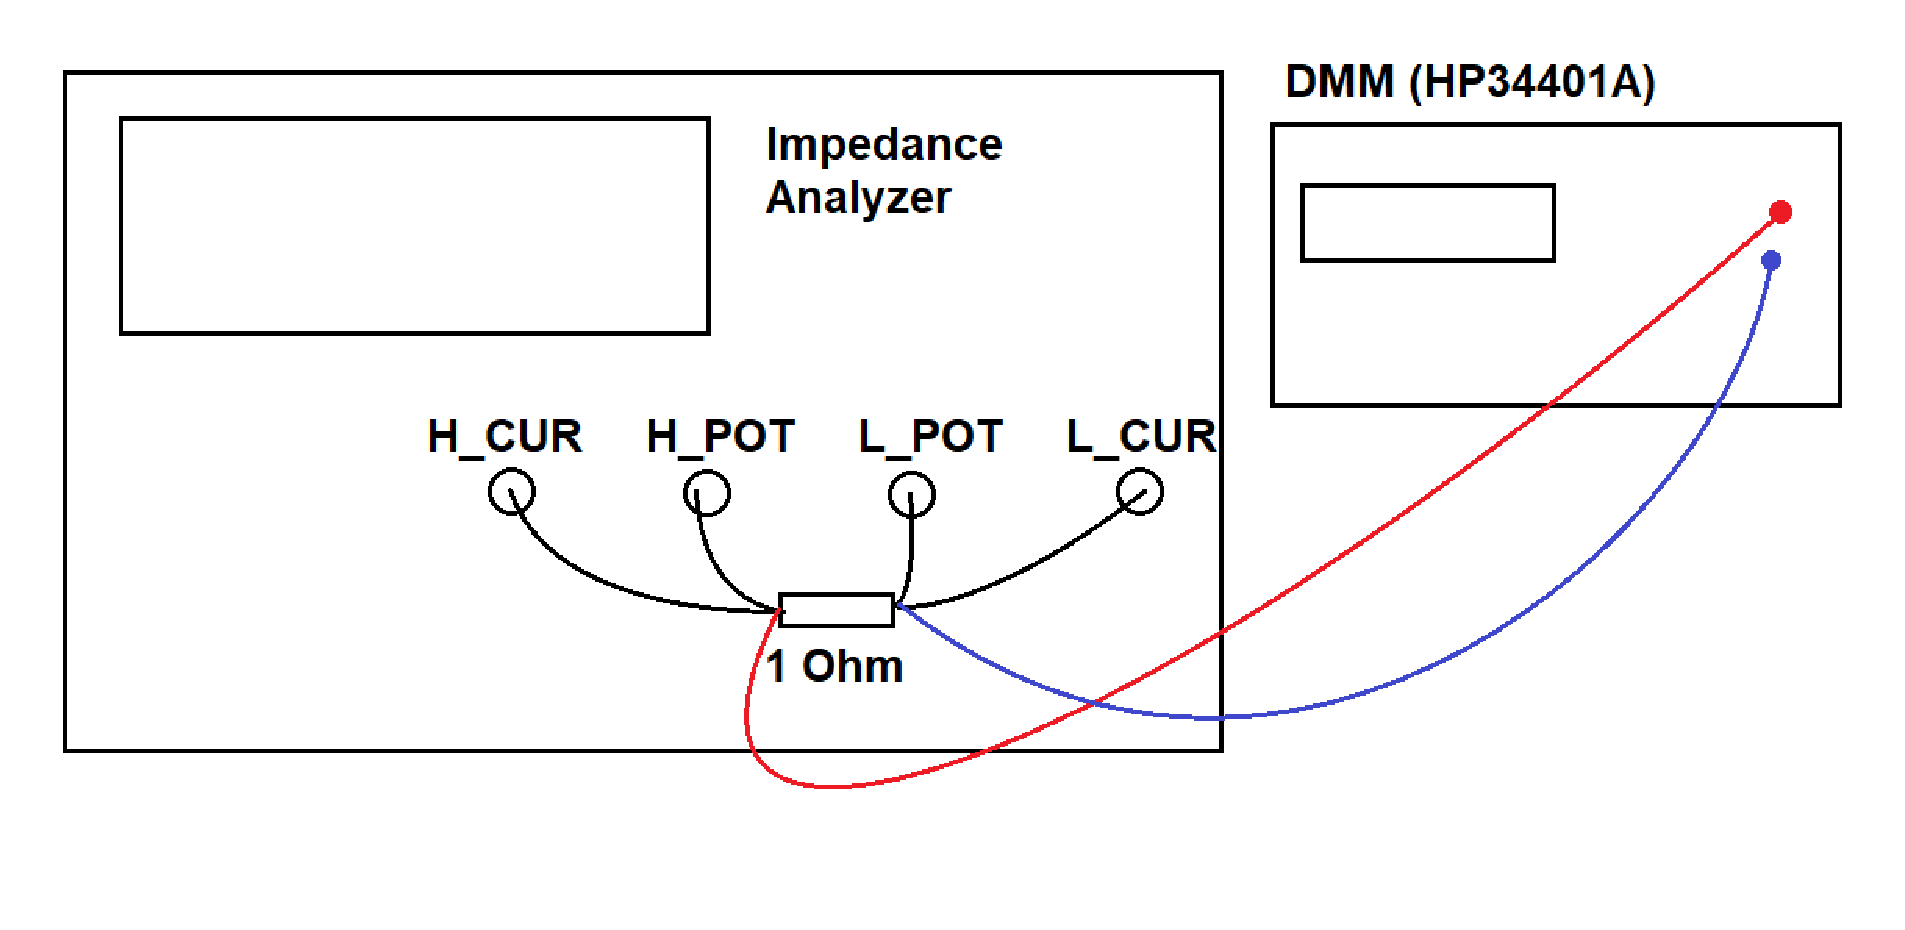
\includegraphics[clip, trim=0 0 0 0, width=0.75\textwidth]{Appendix/Figures/CurrentTest.pdf}
    \caption{The used setup to test of the system can deliver the required amount of current.}
    \label{fig:App_MaxCurrent}
\end{figure}

\subsection*{Result}
The voltage across the resistor was measured to \SIQ{37.172}{\milli\volt}$_{rms}$ or \SIQ{105.14}{\milli\volt}$_{pp}$. This indicates that more than the required test current can be delivered by the Impedance Analyzer, i.e. using a \SIQ{1}{\ohm} resistor the current is \SIQ{105.14}{\milli\ampere}$_{pp}$.



\section{§1 Frequency Range} \label{subsec:BW_Test}
This section describes how the frequency range of the developed system is tested.

The Impedance Analyzer has a differential output. An oscilloscope with two or more channels and a bandwidth of more than \SIQ{50}{\mega\hertz} is used to measure both channels. Channel 1 is connected to $H_{CUR}$ and channel 2 is connected to $L_{CUR}$, these connections should be done using a BNC cable. The oscilloscope is configured for AC inputs, and to display the sum of channel 1 and channel two. The amplitude of the signal is then measured. The test setup can be seen on figure \ref{fig:App_BW_Test}.

The Impedance analyzer is configured to generate \SIQ{2.3}{\volt}$_{pp}$ at \SIQ{50}{\hertz}, \SIQ{1}{\kilo\hertz} and \SIQ{1}{\mega\hertz}. The amplitude at \SIQ{50}{\hertz} and \SIQ{1}{\mega\hertz} should not have decreased by more than \SIQ{-3}{\decibel} compared to the amplitude at \SIQ{1}{\kilo\hertz}.

The system shall then be set for \SIQ{1}{\kilo\hertz} output where the actual output frequency is measured. It shall then be set for \SIQ{1.001}{\kilo\hertz} output and have the output frequency measured.

\begin{figure}[H]
    \centering
    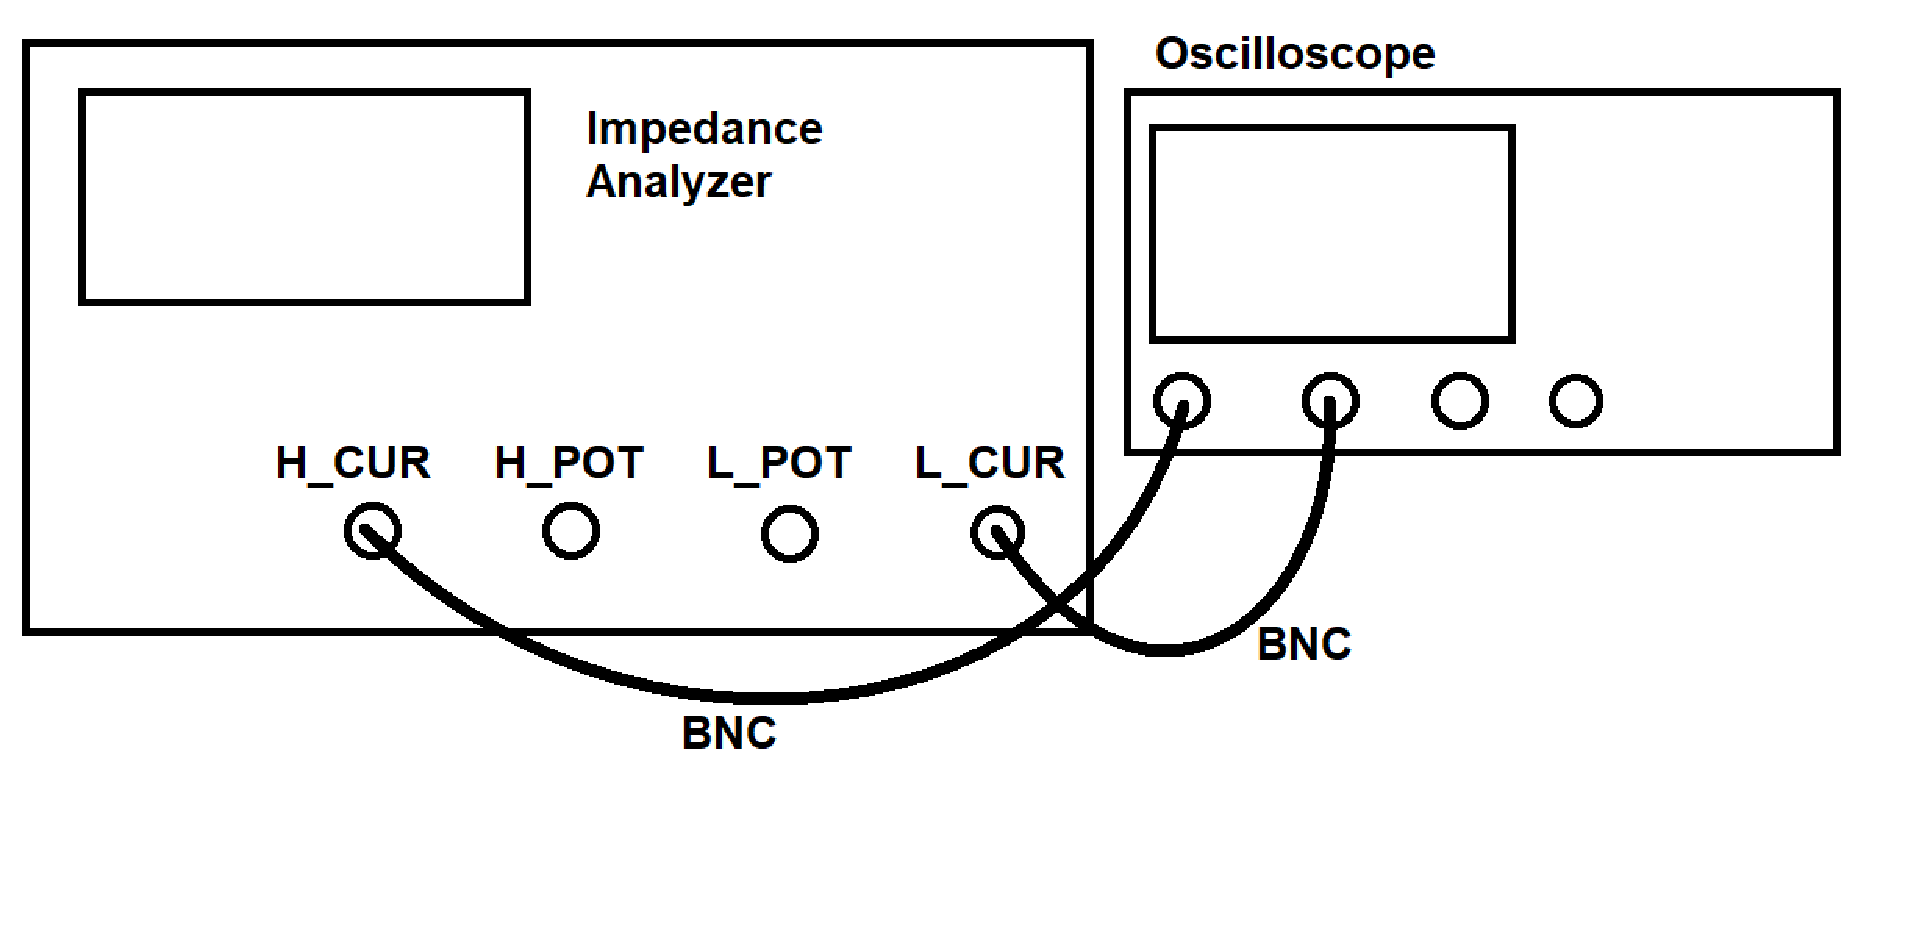
\includegraphics[clip, trim=0 0 0 0, width=0.75\textwidth]{Appendix/Figures/BW_Test.pdf}
    \caption{The used setup to test the frequency range of the Impedance Analyzer.}
    \label{fig:App_BW_Test}
\end{figure}

\subsection*{Result}
\begin{itemize}
    \item \SIQ{1}{\kilo\hertz} amplitude: \SIQ{2.15}{\volt}$_{pp}$
    \item \SIQ{50}{\hertz} amplitude: \SIQ{2.12}{\volt}$_{pp}$ = \SIQ{-0.12}{\decibel}
    \item \SIQ{1}{\mega\hertz} amplitude: \SIQ{2.16}{\volt}$_{pp}$ = \SIQ{0.04}{\decibel}
    \item \SIQ{1.23}{\mega\hertz} amplitude: \SIQ{1.52}{\volt}$_{pp}$ = \SIQ{-3.01}{\decibel}
    \item \SIQ{10}{\hertz} amplitude : \SIQ{1.52}{\volt}$_{pp}$ = \SIQ{-3.01}{\decibel}
    \item --
    \item \SIQ{1.000}{\kilo\hertz} accuracy : \SIQ{1.00001}{\kilo\hertz}
    \item \SIQ{1.001}{\kilo\hertz} accuracy : \SIQ{1.00101}{\kilo\hertz} 
\end{itemize}



The system has a an actual pass-band of \SIQ{10}{\hertz} to \SIQ{1.23}{\mega\hertz}. 

The system can accurately produce a \SIQ{1.000}{\kilo\hertz} sine and a \SIQ{1.001}{\kilo\hertz} sine. This indicates that the resolution is less than \SIQ{1}{\hertz}.